\begin{figure}[h]
    \centering
    \begin{tabular}{c c c c c | c | c}
      Iters=0 & Iters=10 & Iters=50 & Iters=100 & Iters=500 & Iters=1000 & Ground Truth \\
        
\includegraphics[width=0.080\linewidth]{supplementary/cifar/10-0000.png} &
        
\includegraphics[width=0.080\linewidth]{supplementary/cifar/10-0050.png} &
        
\includegraphics[width=0.080\linewidth]{supplementary/cifar/10-0100.png} &
        
\includegraphics[width=0.080\linewidth]{supplementary/cifar/10-0200.png} &
        
\includegraphics[width=0.080\linewidth]{supplementary/cifar/10-0500.png} &
        
\includegraphics[width=0.080\linewidth]{supplementary/cifar/10-1000.png} &
        
\includegraphics[width=0.080\linewidth]{supplementary/cifar/10-ground-truth.png} 
      \\ 
        
\includegraphics[width=0.080\linewidth]{supplementary/cifar/11-0000.png} &
        
\includegraphics[width=0.080\linewidth]{supplementary/cifar/11-0050.png} &
        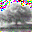
\includegraphics[width=0.080\linewidth]{supplementary/cifar/11-0100.png} &
        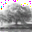
\includegraphics[width=0.080\linewidth]{supplementary/cifar/11-0200.png} &
        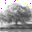
\includegraphics[width=0.080\linewidth]{supplementary/cifar/11-0500.png} &
        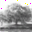
\includegraphics[width=0.080\linewidth]{supplementary/cifar/11-1000.png} &
        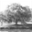
\includegraphics[width=0.080\linewidth]{supplementary/cifar/11-ground-truth.png} 
      \\ 
        
\includegraphics[width=0.080\linewidth]{supplementary/cifar/12-0000.png} &
        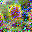
\includegraphics[width=0.080\linewidth]{supplementary/cifar/12-0050.png} &
        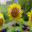
\includegraphics[width=0.080\linewidth]{supplementary/cifar/12-0100.png} &
        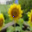
\includegraphics[width=0.080\linewidth]{supplementary/cifar/12-0200.png} &
        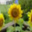
\includegraphics[width=0.080\linewidth]{supplementary/cifar/12-0500.png} &
        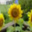
\includegraphics[width=0.080\linewidth]{supplementary/cifar/12-1000.png} &
        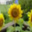
\includegraphics[width=0.080\linewidth]{supplementary/cifar/12-ground-truth.png} 
      \\ 
        
\includegraphics[width=0.080\linewidth]{supplementary/cifar/13-0000.png} &
        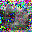
\includegraphics[width=0.080\linewidth]{supplementary/cifar/13-0050.png} &
        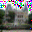
\includegraphics[width=0.080\linewidth]{supplementary/cifar/13-0100.png} &
        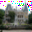
\includegraphics[width=0.080\linewidth]{supplementary/cifar/13-0200.png} &
        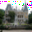
\includegraphics[width=0.080\linewidth]{supplementary/cifar/13-0500.png} &
        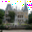
\includegraphics[width=0.080\linewidth]{supplementary/cifar/13-1000.png} &
        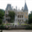
\includegraphics[width=0.080\linewidth]{supplementary/cifar/13-ground-truth.png} 
      \\ 
        
\includegraphics[width=0.080\linewidth]{supplementary/cifar/14-0000.png} &
        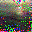
\includegraphics[width=0.080\linewidth]{supplementary/cifar/14-0050.png} &
        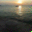
\includegraphics[width=0.080\linewidth]{supplementary/cifar/14-0100.png} &
        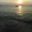
\includegraphics[width=0.080\linewidth]{supplementary/cifar/14-0200.png} &
        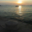
\includegraphics[width=0.080\linewidth]{supplementary/cifar/14-0500.png} &
        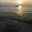
\includegraphics[width=0.080\linewidth]{supplementary/cifar/14-1000.png} &
        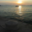
\includegraphics[width=0.080\linewidth]{supplementary/cifar/14-ground-truth.png} 
      \\ 
        
\includegraphics[width=0.080\linewidth]{supplementary/cifar/15-0000.png} &
        
\includegraphics[width=0.080\linewidth]{supplementary/cifar/15-0050.png} &
        
\includegraphics[width=0.080\linewidth]{supplementary/cifar/15-0100.png} &
        \includegraphics[width=0.080\linewidth]{supplementary/cifar/15-0200.png} &
        \includegraphics[width=0.080\linewidth]{supplementary/cifar/15-0500.png} &
        \includegraphics[width=0.080\linewidth]{supplementary/cifar/15-1000.png} &
        \includegraphics[width=0.080\linewidth]{supplementary/cifar/15-ground-truth.png} 
      \\ 
    \end{tabular}
    \caption{The visualization showing the deep leakage on images from MNIST~\cite{lecun1998mnist}, CIFAR~\cite{krizhevsky2009cifar}, SVHN~\cite{netzer2011svhn} and LFW~\cite{LFWTech} respectively. 
    Our algorithm fully recovers the four images while previous work only succeed on images with clean background.
    % More examples can be found in appendix. \zhijian{I think one visualization for the history should be enough; we can put more final results}
    }
    \label{fig:experiment_vision}
\end{figure}